%! Suppress = MissingImport
%! Suppress = TooLargeSection
%! Suppress = SentenceEndWithCapital
%! Suppress = LineBreak
%! Suppress = MissingLabel
%! Suppress = Unicode

\documentclass[main.tex]{subfiles}

\begin{document}
    \setcounter{section}{75}

    \section{Relacyjny model danych, normalizacja relacji (w szczególności algorytm doprowadzenia relacji do postaci
    Boyce’a-Codda), przykłady.}

    \subsection{Relacyjny model danych}
    \begin{itemize}[noitemsep]
        \item Dane w \textbf{tabelach}. Tabela może przedstawiać \textbf{relację bazodanową}.
        \item \textbf{Wiersz (rekord)} - reprezentuje pewną \textbf{encję lub związek}; powinien być
        \textbf{unikalny} wewnątrz tabeli.
        \item \textbf{Atrybuty} - \textbf{kolumny}. Nazwane, mają określony, logicznie niepodzielny typ.
        \item \textbf{Skalar} - pojedyncza wartość, najmniejsza semantycznie jednostka danych; \textbf{atomowy w ramach modelu} relacyjnego.
        \item \textbf{Zmienna relacji} - \textbf{nazwany obiekt, którego wartość zmienia się w czasie}.
        \textbf{Wartość zmiennej} w danej chwili nazywa się \textbf{wartością relacji}.
        \item Relacyjna baza to \textbf{zestaw znormalizowanych relacji różnych stopni}.
        \item  \textbf{Klucz główny} -- minimalna kombinacja pól identyfikująca każdy rekord w tabeli w sposób jednoznaczny.
    \end{itemize}

    \subsection{Relacja bazodanowa}
    Wg Date'a: Relacja R (w znaczeniu \textbf{wartość relacji}) na zbiorze niekoniecznie różnych dziedzin $D_1, D_2,\dots, D_n$
    składa się z dwóch części: \textbf{nagłówka} (heading) i \textbf{treści} (body).\\

    \textbf{Nagłówek} jest to ustalony \textbf{zbiór atrybutów}, tj. zbiór par $<nazwa\_atrybutu :
    nazwa\_dziedziny>$, dziedzina to zbiór wartości skalarnych. Atrybuty \textbf{nie są uporządkowane}.\\

    \textbf{Treść} jest to \textbf{zbiór unikalnych, nieuporządkowanych krotek}, tj. zbiorów par
    $<nazwa\_atrybutu : wartosc\_atrybutu>$ zawierających wszystkie atrybuty z nagłówka.
    \textbf{Posiada przynajmniej jeden klucz kandydujący}.\\

    \noindent \textbf{Liczebność} relacji - liczba krotek w zbiorze.\\
    \noindent \textbf{Stopień relacji} - ilość dziedzin.\\

    \noindent \textbf{Rodzaje} relacji:
    \begin{itemize}[noitemsep]
        \item \textbf{Relacja nazwana} jest \textbf{nazwaną zmienną relacji} zdefiniowana w SZBD.
        \item \textbf{Relacja podstawowa} (autonomiczna) - wystarczająco ważna, by stanowić \textbf{nazwany niezależny byt} w bazie danych. "Przechowuje dane”.
        \item \textbf{Relacja wyprowadzana} (pochodna) - relacja, którą można otrzymać ze zbioru nazwanych relacji za pomoca jakiegoś \textbf{wyrażenia relacyjnego}.
        \item \textbf{Perspektywa} (widok) - nazwana relacja pochodna.
        \item \textbf{Migawka} (snapshot) - rzeczywista nazwana relacja pochodna.
        \item \textbf{Wynik zapytania} - powstaje w wyniku realizacji zapytania.
        \item \textbf{Wynik pośredni} - powstaje w wyniku realizacji podzapytania.
        \item \textbf{Typy}: jeden do jednego, wiele do jednego, wiele do wielu.
    \end{itemize}

    \subsection{Postaci normalne}

    \textbf{Pierwsza postać normalna 1NF}
    \begin{itemize}[noitemsep]
        \item Krotki unikalne, nieuporządkowane, istnieje klucz kandydujący. Atrybuty atomowe, wartości skalarne
        \item \textit{Normalizacja}: wyeliminowania powtarzających się grup -- rozbicie na wartości skalarne.
        \item \textit{Przykład}: atrybut "imiona" wszystkie imiona danej osoby $\rightarrow$ osobne pola na każde imię
    \end{itemize}

    \noindent \textbf{Druga postać normalna 2NF}
    \begin{itemize}[noitemsep]
        \item Żaden niekluczowy (wtórny) atrybut nie jest zależny funkcyjnie od żadnego podzbioru właściwego klucza kandydującego.
        \item Każdy atrybut wtórny jest w pełni zależny funkcyjnie od klucza kandydującego.
        \item \textit{Normalizacja}: wyeliminowanie danych niezależnych od klucza.
        \item \textit{Przykład}: \{Imię, nazwisko, płeć\} $\rightarrow$ \{Imię, nazwisko\} \{Imię, płeć\}.
    \end{itemize}

    \noindent \textbf{Trzecia postać normalna 3NF}
    \begin{itemize}[noitemsep]
        \item \textbf{Żaden atrybut niekluczowy nie jest zależny funkcyjnie od innego atrybutu niekluczowego}.
        \item Dla każdej nietrywialnej zależności funkcyjnej $\{A_1,\dots,A_n\} \rightarrow \{B\}$ zbiór atrybutów $\{A_1,\dots,A_n\}$ jest nadkluczem lub atrybut B jest elementem pewnego klucza kandydującego.
        \item \textit{Normalizacja}: wyeliminowanie danych niezależnych od klucza:
        \begin{enumerate}[noitemsep]
            \item Szukamy wszystkich nietrywialnych, całkowitych zależności funkcyjnych $\{A_1,\dots,A_n\} \rightarrow \{B_i\}$, które naruszają warunek trzeciej postaci normalnej.
            \item Załóżmy, że otrzymujemy zależność (*)$\{A_1,\dots,A_n\} \rightarrow \{B_1, \dots, B_m\}$. Dzielimy schemat relacji na dwa nierozłączne podzbiory:
            \begin{itemize}
                \item Pierwszy, zawierający wszystkie atrybuty występujące w zależności (*).
                \item Drugi, zawierający atrybuty z lewej strony rozważanej zależności (*) oraz atrybuty nie występujące ani z lewej ani z prawej strony tej zależności.
            \end{itemize}
        \end{enumerate}
        \item \textit{Przykład}: \{Imię, Nazwisko, Stanowisko, Stawka\} $\rightarrow$ \{Imię, Nazwisko, Stanowisko\},
        \{Stanowisko, Stawka\}
    \end{itemize}

    \noindent \textbf{Postać normalna Boyce'a-Codda}
    \begin{itemize}[noitemsep]
        \item Dla każdej całkowicie nietrywialnej zależności funkcyjnej $A \rightarrow B$ zbiór \textbf{A jest nadkluczem}.
        \item \textit{Normalizacja}: jak dekompozycja do 3PN. \textbf{Nie zawsze zachowuje zależności funkcyjne}.
    \end{itemize}

    \noindent \textbf{Czwarta postać normalna 4NF}
    \begin{itemize}[noitemsep]
        \item Dla każdej nietrywialnej zależności wielowartościowej X ->> Y \textbf{zbiór X zawiera klucz relacji}.
        \item \textit{Normalizacja}: analogicznie jak dla 3PN.
    \end{itemize}


    \section{Indeksowanie w bazach danych: drzewa B+, tablice o organizacji indeksowej, indeksy haszowe, mapy binarne.}

    \textbf{Indeks} -- \textbf{struktura danych} na dysku umożliwiająca szybkie wyszukiwanie danych w bazie danych
    na podstawie wartości klucza.

    \begin{itemize}[noitemsep]
        \item \textbf{Zaleta} Zmniejszenie czasu odszukania potrzebnych danych (minimalizowanie liczby odczytów bloków danych z dysku)
        \item \textbf{Wada}: Zwiększenie czasu zmiany danych, na których założony jest indeks (zmiana takich danych oznacza zmiane w indeksie)
    \end{itemize}

    \noindent \textbf{Implementacje indeksów}: drzewa B+, tablice haszujące, plik uporządkowany z wyszukiwaniem binarnym.\\

    \noindent \textbf{Typy indeksów (dla plików sekwencyjnych)}
    \begin{itemize}[noitemsep]
        \item \textbf{Główne} (Primary) -- na identyfikatorach wierszy,
        \item \textbf{Drugorzędne} (Secondary) -- pomocnicze.\\

        \item \textbf{Gęste} (Dense) -- każdy wiersz danych ma swój wpis w indeksie,
        \item \textbf{Rzadkie} (Sparse) -- każdy blok danych ma jeden wpis w indeksie. Dane muszą być posortowane według
        klucza indeksu.\\

        \item \textbf{Grupujące} (clustering) – ten termin jest wieloznaczny. W odniesieniu do plików sekwencyjnych
        oznacza grupowanie w jednym bloku \textbf{wierszy z taką samą wartością klucza indeksu}; taki \textbf{indeks}
        budowany jest \textbf{na polu niekluczowym} i wymaga \textbf{posortowania wierszy} według \textbf{pola indeksowanego}.
        \item \textbf{Wielopoziomowe}.
    \end{itemize}


    \section{Podstawowe cechy transakcji (ACID). Metody sterowania współbieżnością transakcji, poziomy izolacji transakcji, przykłady.}

    \subsection{Transakcja}
    Transakcja jest wykonywanym programem, który tworzy logiczną jednostkę przetwarzania w
    bazie danych.\\

    \noindent \textbf{ACID}
    \begin{itemize}[noitemsep]
        \item \textbf{Atomicity} (niepodzielność) -- transakcja wykonywana \textbf{w całości albo wcale}.
        \item \textbf{Consistency} (spójność) po zakończeniu transakcji baza musi być w stanie spójnym, tzn muszą być \textbf{zachowane wszystkie więzy} narzucone na dane.
        \item \textbf{Isolation} (izolacja) wykonywana w \textbf{izolacji od innych} transakcji.
        \item \textbf{Durability} (trwałość) po zakończeniu transacji jej \textbf{efekty} muszą być \textbf{trwałe} w systemie nawet w przypadku awarii.
    \end{itemize}

    \noindent \textbf{Stany transakcji}
    \begin{itemize}[noitemsep]
        \item \textbf{Aktywna} – podczas wykonywania operacji.
        \item \textbf{Częściowo zatwierdzona} – ostatnia operacja transakcji została wykonana. Teraz protokół zatwierdzania musi zapewnić \textbf{trwałość zmian}. Ew. sprawdzenie czy może zostać zatwierdzona. Jeśli może, to osiągnęła swój \textbf{punkt zatwierdzenia}.

        \item \textbf{Nieudana} – wykonywanie transakcji \textbf{nie może być kontynuowane}.

        \item \textbf{Przerwana, wycofana} – baza jest \textbf{odtworzona} do stanu sprzed rozpoczęcia transakcji.
        \item \textbf{Zatwierdzona} – wszelkie \textbf{zmiany} wykonane przez transakcje muszą być \textbf{trwałe}. Zatwierdzonej transakcji \textbf{nie można już wycofać} (ew. \textbf{transakcja kompensująca}).
    \end{itemize}

    \noindent \textbf{Implementacja atomowości i trwałości} -- strategie zarządców buforów:
    \begin{itemize}[noitemsep]
        \item \textbf{Fix} - nie może być zapisów przed końcem transakcji.
        \item \textbf{No-Fix} - mogą być zapisy przed końcem transakcji. Synchronizacja może być realizowana \textbf{cyklicznie} w ramach procesu zwanego \textbf{punktem kontrolnym}.\\

        \item \textbf{Flush} - synchronizacja zmienionych bloków po zakończeniu transakcji.
        \item \textbf{No-Flush} - brak obowiązku synchronizowania zmienionych bloków na koniec transakcji. Synchronizacja może być wykonana później.
    \end{itemize}
    W większości systemów wykorzystujących dzienniki transakcji stosowana jest \textbf{strategia No-Fix/No-Flush}.


    \subsection{Techniki sterowania współbieżnością transakcji}
    Blokady na dane:
    \begin{itemize}[noitemsep]
        \item \textbf{Blokady wyłączne} (typu X, exclusive, blokady do zapisu)
        \item \textbf{Blokady wspólne} (typu S, shared, blokady do odczytu)
    \end{itemize}

    \noindent Blokady na poziomie tabeli:
    \begin{itemize}[noitemsep]
        \item \textbf{IS (intent shared)} – wspólna blokada zapobiegająca – transakcja zamierza założyć blokadę S
        na poszczególnych wierszach tabeli (ogólnie: węzłach potomnych)
        \item \textbf{IX (intent exclusive)} – wyłączna blokada zapobiegająca – zamiar założenia blokady X na
        wierszach (ogólnie: węzłach potomnych)
        \item \textbf{SIX (shared intent exclusive)} – wspólna wyłączna blokada zapobiegająca – na tabeli (węźle
        macierzystym) jest już blokada S, zamierza się założyć blokadę X na wiersze (połączenie S
        oraz IX).
    \end{itemize}

    \begin{table}[H]
        \begin{tabular}{|c|c|c|c|c|c|c| }
            \hline
            Poziom izolacji & P0 & P1 & P2 & P3 & Blokady X & Blokady S \\
            \hline
            Locking READ UNCOMMITED & NIE & TAK & TAK & TAK & długie & nie \\
            \hline
            Locking READ COMMITED & NIE & NIE & TAK & TAK & długie & krótkie\\
            \hline
            Locking REPEATABLE READ & NIE & NIE & NIE & TAK & długie & długie\\
            \hline
            Locking SERIAZABLE & NIE & NIE & NIE & NIE & długie & długie predykatowe\\
            \hline
        \end{tabular}
    \end{table}

    A - oryginalna definicja, P - rozszerzona.\\

    \noindent Dirty Write:
    \begin{center}
        P0: w1[x]...w2[x]...((c1 lub a1) i (c2 lub a2) w dowolnej kolejności)
    \end{center}

    \noindent Dirty Read:
    \begin{center}
        P1: w1[x]...r2[x]...((c1 lub a1) i (c2 lub a2) w dowolnej kolejności)\\
        A1: w1[x]...r2[x]...(a1 i c2 w dowolnej kolejności)\\
    \end{center}


    \noindent Non-rep or Fuzzy Read:
    \begin{center}
        P2: r1[x]...w2[x]...((c1 lub a1) i (c2 lub a2) w dowolnej kolejności)\\
        A2: r1[x]...w2[x]...c2...r1[x]...c1\\
    \end{center}


    \noindent Phantom:
    \begin{center}
        P3: r1[P]...w2[y in P]...((c1 lub a1) i (c2 lub a2) w dowolnej kolejności)\\
        A3: r1[P]...w2[y in P]...c2...r1[P]...c1\\
    \end{center}


    \noindent Lost update:
    \begin{center}
        P4: r1[x]...w2[x]…c2 ...w1[x]...c1
    \end{center}

    \subsection{Wielowersyjne techniki sterowania współbieżnością}

    \textbf{Poziom izolacji Cursor Stability} -- rozszerzenie sposobu blokowania w poziomie Locking READ COMMITTED.
    \begin{itemize}[noitemsep]
        \item operacja \textbf{rc (czytaj kursor, pobierz wiersz)} dla instrukcji FETCH, blokada (S lub nowy typ
        blokady do odczytu \textbf{scroll lock}) będzie utrzymywana \textbf{do chwili przejścia} do innego wiersza lub
        do \textbf{zamknięcia} kursora.
        \item operacja \textbf{wc (write cursor)} powoduje założenie na ten wiersz \textbf{długiej blokady X}.
    \end{itemize}

    Nowa odmiana problemu P4:
    \textbf{P4C: rc1[x]...w2[x]...c2...wc1[x]...c1}\\

    \noindent Poziom izolacji Cursor Stability \textbf{eliminuje P4C}, w2[x] będzie wstrzymane do zdjęcia blokady (S, scroll lock) przez przejście do innego wiersza lub zamknięcie kursora.\\

    \noindent \textbf{Poziom izolacji Snapshot} -- \textbf{transakcja czyta dane (zatwierdzone) z chwili swojego początku}, Start-Timestamp.

    Protokoły odczytu spójnych wersji czasowych.
    \begin{itemize}
        \item \textbf{Snapshot isolation v1} -- wszelkie zmiany są wykonywane na lokalnych kopiach i zapisywane na
        końcu transakcji. Aktualizacje wykonywane przez inne transakcje nie są odczytywane.
        \item \textbf{Snapshot isolation v2} -- blokady do zapisu, ponadto przy każdym zapisie
        transakcja wykonuje sprawdzenie czy ma aktualne dane.
        \item \textbf{Read Committed Snapshot} (Read Consistency) -- operacja odczytu czyta ostatnią zatwierdzoną (aktualną)
        wartość elementu danych.
    \end{itemize}


    \section{Złączenia, grupowanie, podzapytania w języku SQL.}

    \textbf{JOIN} -- łączenie tabel między kluczem podstawowym i kluczem obcym drugiej.
    \begin{itemize}[noitemsep]
        \item Łączenia \textbf{wewnętrzne} -- \texttt{INNER JOIN} -- wybiera rekordy posiadające takie same wartości w
        obu tabelach.
        \item Łączenia \textbf{zewnętrzne} -- \texttt{LEFT/RIGHT/FULL OUTER JOIN} -- zwraca $L \cap R$/$R \cap L$/$L \cup R$.
    \end{itemize}

    \noindent \textbf{GROUP BY} -- tworzenie grup rekordów w oparciu o definicję grupowania, wykonywane po filtrowaniu.\\

    W przypadku stosowania GROUP BY, w trakcie przetwarzania zapytania, tworzone są dwie sekcje danych.
    \begin{itemize}[noitemsep]
        \item \textbf{Sekcja grupująca} składa się z atrybutów tworzących definicję grupowania.
        \item \textbf{Sekcja danych surowych} (raw data section) zawierają wszystkie pozostałe dane.
    \end{itemize}

    \noindent \textbf{Podzapytania} -- instrukcje SELECT wewnątrz innej instrukcji SELECT. Serwer bazodanowy w pierwszej
    kolejności wykona zapytania wewnętrzne. Wynik zapytania wewnętrznego zwracany jest do zapytania zewnętrznego.

    \begin{itemize}
        \item podzapytania \textbf{niepowiązane} (nieskorelowane) -- wykonywane tylko raz, zwraca jeden wynik;
        może być wykonane samodzielnie; często używane w WHERE.
        \item podzapytania \textbf{powiązane} (skorelowane) -- bezpośrednio powiązane z zapytaniem nadrzędnym poprzez
        przekazywane przezeń atrybuty; wykonywane osobno dla każdego wiersza; używane do wyliczenia nowego atrybutu.
    \end{itemize}


    \section{Szeregowalność harmonogramów w bazach danych.}

    \textbf{Harmonogram} - inaczej historia S zbioru n transakcji $T_1, \dots, T_n$ jest takim ciągiem wszystkich
    operacji transakcji, że dla każdej transakcji $T_i \in S$ operacje tej transakcji w S muszą występować w takiej samej
    kolejności, w jakiej występują w $T_i$. Operacje z różnych transakcji mogą się przeplatać.

    \begin{itemize}[noitemsep]
        \item \textbf{Harmonogram szeregowy} - operacje każdej transakcji są wykonywane kolejno, \textbf{bez przeplatania}
        operacji z różnych transakcji. Są nieefektywne.
        \item \textbf{Harmonogram szeregowalny} - jego wpływ na stan bazy danych jest taki sam jak pewnego
        harmonogramu szeregowego.
        \item \textbf{Harmonogram nieszeregowy} - harmonogram, który nie jest sekwencyjny.
        \item \textbf{Harmonogram pełny} - harmonogram zawierający wszystkie operacje z transakcji składowych, gdzie dla
        dowolnych dwóch \textbf{operacji}, które są w \textbf{konflikcie}, jedna z nich musi \textbf{poprzedzać} drugą
        w harmonogramie.
    \end{itemize}

    \noindent \textbf{Konflikt operacji} -- wie operacje są w stanie konfliktu, jeśli spełnione są warunki:
    \begin{itemize}[noitemsep]
        \item Należą do \textbf{różnych transakcji},
        \item Uzyskują dostęp do \textbf{tego samego elementu},
        \item \textbf{Przynajmniej jedna} z operacji jest \textbf{operacją zapisu} elementu.
    \end{itemize}

    \begin{itemize}
        \item \textbf{Równoważność konfliktowa} -- jeżeli \textbf{kolejność} wszystkich \textbf{operacji konfliktowych}
        jest w obu harmonogramach \textbf{taka sama}. Wyniki harmonogramów równoważnych konfliktowo są takie same.
        \item \textbf{Szeregowalność konfliktowa} -- jeżeli harmonogram S jest \textbf{konfliktowo równoważny} pewnemu
        harmonogramowi \textbf{szeregowemu} S’. Możemy zmieniać kolejność niekonfliktowych operacji w S.
        \textbf{Warunek wystarczający zachowania spójności danych}.\\

        \item \textbf{Równoważność perspektywiczna harmonogramów}. Harmonogram S i S' zawierają te same instrukcje i dla każdego
        elementu danych Q:
        \begin{itemize}
            \item Jeśli $T_k$ jest transakcją, która w
            S czyta Q jako pierwsza, to w S' $T_k$ musi być transakcją, która czyta Q jako pierwsza.
            \item Jeśli w S $T_i$ czyta Q zapisany przez $T_j$, to w S' $T_i$ czyta Q zapisany przez $T_j$.
            \item Jeśli w S  $T_m$ jest ostatnią transakcją, która
            zapisuje Q, to w S' $T_m$ jest ostatnią transakcją, która zapisuje Q.
        \end{itemize}

        \item \textbf{Szeregowalność perpektywiczna}. Harmonogram szeregowalny perspektywicznie jest harmonogramem
        \textbf{równoważnym perspektywicznie} jakiemuś harmonogramowi szeregowemu.

        Szeregowalność perspektywiczna to \textbf{szeregowalność konfliktowa z dodatkowymi ograniczeniami} operacji zapisów:
        \begin{itemize}
            \item każda operacja w(x) jest poprzedzona r(x),
            \item wartość zapisana przez operację w(x) \textbf{jest nie-stałą funkcją} zależną tylko od wartości r(x).
        \end{itemize}
    \end{itemize}


    \section{Definicja cyfrowego układu kombinacyjnego - przykłady układów kombinacyjnych i ich implementacje.}

    \textbf{Układ kombinacyjny} to taki układ logiczny, w którym \textbf{każda kombinacja wartości zmiennych wejściowych
    jednoznacznie określa kombinację wartości zmiennych wyjściowych}. Opisujemy je za pomocą bramek logicznych
    lub tablicy prawdy.

    \textbf{Bramka logiczna} to układ elektroniczny realizujący funkcję logiczną jednej lub wielu zmiennych
    (w podstawowej wersji dwóch).

    \textbf{Półsumator (Half Adder).}

    \begin{figure}[H]
        \includegraphics[width=\linewidth]{uk/ha.png}
    \end{figure}

    \begin{tabular}{c c}
        \includegraphics[width=0.5\linewidth]{uk/ha_l.png}
        &
        \begin{tabular}{c}
            $s(x,y) = \sum (1,2) = \bar{x}y + x\bar{y} = x \oplus y$\\
            $c(x,y) = \sum (3) = xy$
        \end{tabular}
    \end{tabular}
    \hfill \\

    \noindent \textbf{Sumator (Full Adder).}

    \begin{tabular}{c c}
        \includegraphics[width=0.4\linewidth]{uk/fa.png}
        &
        \begin{tabular}{c}
            $s(x,y) = \sum (1,2,4,7) = \bar{x}\bar{y}z + \bar{x}y\bar{z} + xyz$\\
            $c(x,y) = \sum (3,5,6,7) = xz + yz + xy$\\
            \includegraphics[width=0.5\linewidth]{uk/fa_l.png}
        \end{tabular}
    \end{tabular}
    \hfill \\

    \noindent \textbf{Dekoder} -- układ kombinacyjny mający $n$ wejść i $m \leq 2^n$ wyjść, w którym każdej kombinacji
    zmiennych wejściowych odpowiada pojawienie się jedynki logicznej tylko na jednym wyjściu, na pozostałych wyjściach zera.

    \begin{figure}[H]
        \includegraphics[width=\linewidth]{uk/dek.png}
    \end{figure}

    \textbf{Koder to układ kombinacyjny działający odwrotnie do dekodera}.
    \hfill \\

    \noindent \textbf{Multiplekser} -- układ kombinacyjny wybierający informację dwójkową na jednej z linii wejściowych i kierujący
    ją na jedną linię wyjściową. Wybór linii wejściowej jest określany przez linie sterujące.

    \begin{figure}[H]
        \includegraphics[width=\linewidth]{uk/mul.png}
    \end{figure}

    \begin{figure}[H]
        \includegraphics[width=\linewidth]{uk/mul_l.png}
    \end{figure}


    \section{Definicja cyfrowego układu sekwencyjnego - przykłady układów sekwencyjnych i ich implementacje.}

    \textbf{Układ sekwencyjny} -- układ, w którym poziomy sygnałów wyjściowych zależą nie tylko od wejścia
    ale również od stanu poziomów, które występowały uprzednio.
    Oznacza to, że układy te zawierają elementy pamiętające i nazywane są czasem \textbf{układami kombinacyjnymi z pamięcią}.

    \subsection{Przerzutnik RS (Reset-Set)}
    \begin{itemize}[noitemsep]
        \item najprostrzy przerzutnik: 2xNOR.
        \item $R \rightarrow \overline{Q}$, $S \rightarrow \overline Q_n$ tylko jeśli na którymś sygnał.
    \end{itemize}

    \begin{table}[H]
        \center
        \begin{tabular}{p{8cm} p{8cm}}
            \begin{tabular}{|c|c|c|c|}
                \hline
                \textbf{R} & \textbf{S} & $Q_n$ & $\overline{Q_n}$ \\ \hline \hline
                0 & 0 & $Q_{n-1}$ & $\overline{Q_{n-1}}$            \\ \hline
                0 & 1 & 1 & 0              \\ \hline
                1 & 0 & 0 & 1              \\ \hline
                1 & 1 & - & -              \\ \hline
            \end{tabular}
            &
            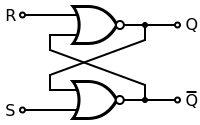
\includegraphics[width=0.5\linewidth]{sequentials/rs.png}
        \end{tabular}
    \end{table}


    \subsection{Przerzutnik D (Delay)}
    \begin{itemize}[noitemsep]
        \item wejścia D oraz C (Clock)
        \item D przechodzi na wyjście w momencie ``tyknięcia'' zegara -- przerzutnik jest \textbf{synchroniczny}
    \end{itemize}

    \begin{table}[H]
        \center
        \begin{tabular}{p{8cm} p{8cm}}
            \begin{tabular}{|c|c|c|c|}
                \hline
                \textbf{D} & $\mathbf{Q_{n-1}}$ & $\mathbf{Q_n}$ \\ \hline
                0 & - & 0              \\ \hline
                1 & - & 1              \\ \hline
            \end{tabular}
            &
            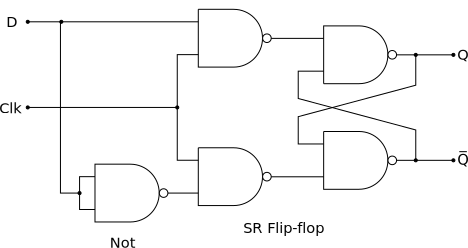
\includegraphics[width=0.5\linewidth]{sequentials/d.png}
        \end{tabular}
    \end{table}

    \subsection{Przerzutnik JK}
    \begin{itemize}[noitemsep]
        \item synchroniczny,
        \item obsługuje stan 11,
        \item  3 wejścia: J(S), K(R) oraz Clock, wyjście: Q -- stałe dla 00, odwrotne dla 11, równe J wpp.
    \end{itemize}

    \begin{table}[H]
        \center
        \begin{tabular}{p{8cm} p{8cm}}
            \begin{tabular}{|c|c|c|c|}
                \hline
                \textbf{J} & \textbf{K} & $\mathbf{Q_{n-1}}$ & $\mathbf{Q_n}$ \\ \hline
                0 & 0 & 0 & 0              \\ \hline
                0 & 0 & 1 & 1              \\ \hline
                1 & 0 & - & 1              \\ \hline
                0 & 1 & - & 0              \\ \hline
                1 & 1 & 0 & 1              \\ \hline
                1 & 1 & 1 & 0              \\ \hline
            \end{tabular}
            &
            \includegraphics[width=0.5\linewidth]{sequentials/jk.png}
        \end{tabular}
    \end{table}


    \section{Minimalizacja funkcji logicznych.}

    \textbf{Minimalizacja z wykorzystaniem algebry Boole'a} -- polega na \textbf{zapisaniu funkcji w postaci sumy stanów wejść},
    dla których funkcja przyjmuje wratość 1, a następnie wykorzystując prawa algebry Boole'a \textbf{uproszczenie} jej.\\

    \noindent \textbf{Minimalizacja z wykorzystaniem tablic Karnaugha}\\
    \textbf{Tablica Karnaugha} jest cykliczna; składa się z pól reprezentujących wszystkie kombinacje zmiennych naszej
    funkcji, z czego każde sąsiednie dwa pola różnią się jednym bitem.

    \begin{center}
        Dla dwóch zmiennych \\
        \includegraphics[width=\linewidth]{karnaugh/2-vars.png}

        Dla trzech zmiennych \\
        \includegraphics[width=\linewidth]{karnaugh/3-vars.png}
    \end{center}
    Przy pomocy tablic Karnaugha możemy minimalizować funkcję o maksymalnie 6 zmiennych.


    \section{Programowalne układy logiczne PLD (ROM, PAL, PLA).}

    \textbf{ROM (Read Only Memory)}
    \[ k \text{ linii adresowych} \rightarrow 2^k \text{ słów n-bitowych} \rightarrow n \text{ linii wyjściowych}\]
    Zbudowana z dekodera i bramek OR. Jeśli chcemy np. sumator, to wejście do dekodera do xyz, wyjście z dekodera
    to wartości na s i c realizowane przy pomocy OR.\\

    \noindent \textbf{PLA (Programmable Logic Array)} zawierają część programowalną matrycę bramek OR oraz programowalną
    matrycę bramek AND - tzn. realizuje funkcje będące sumą iloczynów, możemy ustawić jakich iloczynów.\\

    \noindent \textbf{PAL (Programmable Array Logic)} -- zawierają część nieprogramowalną (wbudowane bramki OR) oraz programowalną
    matrycę bramek AND -- tak jak PAL, ale \textbf{ustalona ilość OR}.

    \begin{center}
        \begin{tabular}{| c | c |}
            \hline
            \textbf{PLA} & \textbf{PAL}\\
            \hline
            droższe & szybsze\\
            dowolna ilość bramek & ustalona ilość OR\\
            dużo funkcji & ograniczona ilość, bo mniej elastyczne\\
            \hline
        \end{tabular}
    \end{center}


    \section{Schemat blokowy komputera (maszyna von Neumanna).}

    \begin{itemize}[noitemsep]
        \item Niemalże wszystkie cyfrowe, elektroniczne współczesne komputery są oparte na architekturze von Neumanna
        \item Architektura von Neumanna pozwoliła na oddzielenie programu od procesora
        \item Istnieje architektura Harvardzka, oddzielająca pamięć z rozkazami od pamięci z danymi.
        \item Cechy:
        \begin{itemize}[noitemsep]
            \item Jednolitość pamięci:
            \begin{itemize}
                \item Możliwość uruchomienia samomodyfikującego się programu
                \item Dzielenie pamięci instrukcji z pamięcią danych może prowadzić do bottlenecków (w tym celu wprowadza się cache)
            \end{itemize}
            \item Skończona liczba rozkazów
            \item Informacje są przetwarzane poprzez sekwencyjny odczyt kolejnych instrukcji z pamięci i ich wykonanie przez procesor
        \end{itemize}
    \end{itemize}

    \begin{table}[H]
        \begin{center}
            \begin{tabular}{p{6cm} p{11cm}}
                \raisebox{-\height}{\includegraphics[width=6cm]{von_neumann.png}}
                &
                \begin{itemize}
                    \item \textbf{Pamięć} - zawiera zarówno dane, jak i instrukcji
                    \item \textbf{Procesor} (CPU, Central Processing Unit)
                    \begin{itemize}
                        \item \textbf{Jednostka kontrolna} (nadzorująca)
                        \item \textbf{Jednostka arytmetyczno-logiczna} -- wykonuje podstawowe operacje przetwarzania informacji.
                        \begin{itemize}
                            \item \textbf{Akumulator} -- obsługuje urządzenia wejścia/wyjścia (I/O).
                        \end{itemize}
                    \end{itemize}
                \end{itemize}
            \end{tabular}
        \end{center}
    \end{table}


    \section{Zarządzanie procesami: stany procesu, algorytmy szeregowania z wywłaszczaniem.}

    \textbf{Program} to zbiór instrukcji, element procesu znajdujący się w segmencie kodu, którego stan nie ulega
    modyfikacji w czasie wykonywania; wykorzystuje dodatkowe zasoby (procesor, pamięć itp).\\

    \noindent \textbf{Proces} służy do \textbf{organizowania wykonywania programu} w ten sposób, że stanowi on powiązanie
    \textbf{niezbędnych zasobów systemu komputerowego} i umożliwia \textbf{kontrolę stanu} tych zasobów związaną z
    wykonywaniem programu.\\

    \noindent \textbf{Zarządzanie procesami}. Fragmenty kodu jądra związane z obsługą procesów:
    \begin{itemize}[noitemsep]
        \item \textbf{zarządcy procesów} -- grupują i wykonuja funkcje obsługi procesów.
        \item \textbf{zarządcy zasobów} -- kontrolują stan zajętości zasobów i realizację żądań procesów.
    \end{itemize}

    \noindent \textbf{Stany procesu} -- Nowy $\rightarrow$ Gotowy $\leftrightarrow$ Wykonywany
    ($\leftrightarrow$ Oczekujący) $\rightarrow$ Zakończony
    \begin{itemize}[noitemsep]
        \item \textbf{Nowy} — formowanie procesu -- gromadzenie zasobów (z wyjątkiem procesora),
        oczekiwanie na przyjęcie do kolejki procesów gotowych.

        \item \textbf{Gotowy} — oczekiwanie na przydział kwantu czasu procesora

        \item \textbf{Wykonywany} — wykonywanie instrukcji programu danego procesu i wynikająca z ich wykonywania zmiana
        stanu odpowiednich zasobów systemu.

        \item \textbf{Oczekujący} — zatrzymanie wykonywania instrukcji programu ze względy na potrzebę przydziału
        dodatkowych zasobów, konieczność otrzymania danych lub osiągnięcia odpowiedniego stanu przez otoczenie procesu

        \item \textbf{Zakończony} — zakończenie wykonywania programu, zwolnienie większości zasobów i oczekiwanie na
        możliwość przekazania informacji o zakończeniu.
        Pozostawanie procesu z stanie zakończony (zombi) spowodowane jest przetrzymywaniem pewnych informacji o
        procesie po jego zakończeniu (np. statusu).
    \end{itemize}

    \noindent \textbf{Wywłaszczenie} -- przejście Wykonywany $\rightarrow$ Gotowy -- może być następstwem:
    \begin{enumerate}[noitemsep]
        \item \textbf{Upływu kwantu czasu} -- przy algorytmi rotacyjnym planowania przydziału procesora.
        \item \textbf{Pojawienia się procesu gotowego z wyższym priorytetem} -- w systemie z \textbf{dynamicznymi
        priorytetami}, które są przeliczane co jakiś czas, przy stosowaniu wywłaszczeniowego podejścia do planowania
        przydziału procesora.
    \end{enumerate}


    \noindent \textbf{Szeregowanie procesów} (planowanie) -- wybór jednego z procesów (lub wątków) gotowych i
    przekazaniu mu procesora.
    \begin{itemize}[noitemsep]
        \item \textbf{Funkcja priorytetu} (wyboru) wyznacza aktualny priorytet procesu na podstawie parametrów procesu i stanu
        systemu.
        \begin{itemize}[noitemsep]
            \item zbiór wytycznych dla planisty,
            \item w Windows większy = wyższy, w unix mniejszy = wyższy
            \item uwzględnia przede wszystkim stan procesu, może też stan systemu
        \end{itemize}

        \item \textbf{Tryb decyzji} -- kiedy są oceniane priorytety oraz dokonywany jest wybór.
        \begin{itemize}[noitemsep]
            \item zbiórem wytycznych odnośnie uruchamiania ekspedytora,
            \item \textbf{wywłaszczeniowy} lub \textbf{niewywłaszczeniowy} (proces może się zrzec, np. po wejściu w stan oczekiwania).
        \end{itemize}

        \item \textbf{Reguła arbitrażu} — reguła rozstrzygania konfliktów w dostępie do procesora.
        \begin{itemize}[noitemsep]
            \item \textbf{Arbitraż losowy} przy małej zmienności priorytetów mógłby prowadzić do głodzenia procesów.
            \item \textbf{Arbitraż cykliczny} -- trudny w realizacji przy zmiennych priorytetach, ok przy stałych.
            \item \textbf{Arbitraż chronologiczny} (FIFO przyjmowania procesów do systemu) -- najbardziej sprawiedliwy, ale wymaga utrzymania odpowiednich
            atrybutów procesów.
        \end{itemize}
    \end{itemize}


    \noindent \textbf{Algorytmy planowania przydziału procesora}:
    \begin{itemize}
        \item \textbf{FCFS} (First Come First Served)
        \begin{itemize}[noitemsep]
            \item w systemach obsługi masowej, takich jak kasy sklepowe, banki itd.
            \item możliwość oddania procesora innemu procesowi na czas oczekiwania.
        \end{itemize}

        \item \textbf{LCFS} (Last Come First Served)
        \begin{itemize}[noitemsep]
            \item nie wywłaszcza,
            \item nie ma praktycznego zastosowania.
        \end{itemize}

        \item \textbf{SJF} (Shortest Job First)
        \begin{itemize}
            \item preferuje procesy, które mają najmniejsze wymagania odnośnie czasu procesora,
            \item "najpierw zadanie z najkrótszą następną fazą procesora",
            \item równeiż w systemach masowej obsługi,
            \item problem określenia przyszłego zapotrzebowania na procesor.
        \end{itemize}
    \end{itemize}


    \section{Muteks, semafor, monitor jako narzędzia synchronizacji procesów.}
    \textbf{Sekcje krytyczne} -- fragmenty kodu, które nie mogą zostać wykonane „w tym samym czasie” przez kilka wątków.\\

    \noindent \textbf{Semafor} -- chroniona zmienna.
    \begin{itemize}
        \item \textbf{Semafor binarny} przyjmuje wartości \textbf{true} (stan podniesienia, otwarcia) lub
        \textbf{false} (stan opuszczenia, zamknięcia).
        \item \textbf{Semafor ogólny} (zliczający) przyjmuje wartości całkowite nieujemne, zwiększany/zmniejszamy
        przy podniesieniu (V)/opuszczeniu (P).
    \end{itemize}

    \noindent \textbf{Muteks (Zamek)} -- szczególny rodzaj semaforów binarnych (1 - zablokowany, 0 - odblokowany), tylko
    jeden wątek może być w posiadaniu muteksa.

    \begin{itemize}[noitemsep]
        \item \textbf{Cecha posiadania} - jeżeli zadanie zablokuje mutex to tylko ono może ten muteks odblokować.
        \item \textbf{Rekurencyjne blokowanie} - określa ile razy zadanie, które posiada dany muteks wykonało na nim
        operacje blokowania (zapobiega to zakleszczeniu).
    \end{itemize}

    \noindent Operacje:
    \begin{itemize}[noitemsep]
        \item \textbf{lock} (mutex\_lock) -- zajęcie muteksu jeśli jest wolny
        \item \textbf{unlock} (mutex\_unlock) -- ustawienie zamka na wolny lub ustawienie wątku z kolejki na gotowy
        \item \textbf{trylock} (mutex\_trylock) -- zajęcie zamkna lub kontynuacja przetwarzania
    \end{itemize}

    \noindent \textbf{Monitor} (zmienna warunkowa) -- zmienne i działające na nich procedury zebrane w jednym module
    (klasie), dostęp do nich tylko za pomocą procedur. W danej chwili tylko jeden proces może wykonywać procedury
    monitora (FIFO); istnieje możliwość wstrzymania i wznowienia procedur za pomocą zmiennych warunkowych.
    Może to być np. klasa reprezntująca konto w banku i udostępniająca procedury zmiany stanu.

    \noindent Operacje:
    \begin{itemize}[noitemsep]
        \item \textbf{wait} -- powoduje wstrzymanie procesu i wstawienie go na koniec kolejki
        \item \textbf{signal} -- powoduje wznowienie pierwszego procesu z kolejki, o ile kolejka nie jest pusta
    \end{itemize}


    \section{Pamięć wirtualna i mechanizm stronicowania.}

    \textbf{Pamięć wirtualna} jest \textbf{organizacją zasobów pamięci}, zrealizowaną w oparciu o tzw. przestrzeń
    wymiany w pamięci drugiego rzędu (na dysku). Pamięć operacyjna (fizyczna) jest dla tych zasobów tylko pewnym oknem,
    przechowującym część zawartości na potrzeby bieżącego przetwarzania. Stosowanie pamięci wirtualnej umożliwia
    \textbf{bardziej racjonalne wykorzystanie pamięci operacyjnej}, gdyż programy tworzone są często z nadmiarem
    w stosunku do typowych potrzeb.\\

    \noindent \textbf{Stronicowanie}
    \begin{itemize}[noitemsep]
        \item \textbf{Arbitralny podział pamięci fizycznej na ramki}, w które ładowane są odpowiednie strony obrazu procesu.
        \item \textbf{Podział logicznej przestrzeni adresowej na strony} o takim samym rozmiarze, jak ramki w pamięci fizycznej.
        \item \textbf{Zalety}:
        \begin{itemize}[noitemsep]
            \item brak problemu fragmentacji zewnętrznej
            \item wspomaganie dla współdzielenia i ochrony pamięci
        \end{itemize}
        \item \textbf{Wady}:
        \begin{itemize}[noitemsep]
            \item narzut czasowy przy transformacji adresu
            \item narzut pamięciowy (na potrzeby tablicy stron)
            \item fragmentacja wewnętrzna (niewielka)
        \end{itemize}
    \end{itemize}

    \noindent \textbf{Mechanizm stronicowania na żądanie} -- strony są sprowadzane do pamięci tylko wówczas, gdy następuje
    odniesienie do komórki o adresie znajdującym się na tej stronie. Jest przede wszystkim z wymianą stron pomiędzy
    pamięcią pierwszego rzędu (operacyjną, fizyczną) i drugiego rzędu (masową, dyskową).\\

    \noindent \textbf{Problemy zastępowania stron}
    \begin{itemize}[noitemsep]
        \item \textbf{Problem wyboru ofiary} — niewłaściwy wybór ramki-ofiary powoduje wzrost kosztu wymiany.
        W skrajnym przypadku może dojść do zjawiska migotania (częste odnoszenie się do usuniętej strony).
        \begin{itemize}[noitemsep]
            \item Zakładając, że przyszły ciąg odniesień do pamięci nie jest znany, na podstawie \textbf{historii}
            odniesień należy wybrać najlepszą ramkę.
            \item Podstawowa własność programów, na podstawie której można szacować takie prawdopodobieństwo,
            nazywana jest \textbf{lokalnością}.
        \end{itemize}

        \item \textbf{Problem wznawiania rozkazów} — w przypadku wielokrotnego odniesienia do pamięci w jednym cyklu
        rozkazowym należy zapewnić, że wszystkie adresowane strony są jednocześnie dostępne w ramkach w pamięci fizycznej.
    \end{itemize}


    \noindent Klasyfikacja algorytmów wymiany z względu na \textbf{okoliczności sprowadzania i usuwania stron}:
    \begin{itemize}
        \item \textbf{Algorytmy wymiany na żądanie} -- sprowadzanie i usuwanie odbywa się na żądanie (odwołanie/brak
        wolnej ramki)
        \begin{itemize}[noitemsep]
            \item \textbf{MIN} — zastępowana jest strona, która najdłużej nie będzie używana,
            \item \textbf{FIFO} -- First In First Out,
            \item \textbf{LIFO} -- Last In First Out,
            \item \textbf{LRU} -- Least Recently Used,
            \item \textbf{LFU} -- Least Frequently Used,
            \item \textbf{MFU} -- Most Frequently Used.
        \end{itemize}
        \item \textbf{Algorytmy wymiany ze sprowadzaniem na żądanie} -- tylko sprowadzanie dobywa się na żądanie
        \item \textbf{Algorytmy wstępnego sprowadzania} -- sprowadzana jest strona żądana, a wraz z nią inne strony
    \end{itemize}

    \noindent Klasyfikacja algorytmów wymiany ze względu na \textbf{sposób zastępowania stron}
    \begin{itemize}[noitemsep]
        \item \textbf{Zastępowanie lokalne} -— zastępuje tylko strony w ramkach przydzielonych procesowi,
        który spowodował błąd strony.
        \item \textbf{Zastępowanie globalne} —- zastępuje strony znajdujące się w dostępnej puli ramek w
        całym systemie (w szczególności zatem usuwa strony innych procesów).
    \end{itemize}

    \noindent Klasyfikacja algorytmów wymiany ze względu na \textbf{przydział ramek dla procesów}: przydział
    \textbf{statyczny} lub \textbf{globalny}. \textbf{Dobór liczby ramek}:
    \begin{itemize}[noitemsep]
        \item \textbf{Minimalna liczba ramek} — zdefiniowana przez architekturę komputera (zależna od maksymalnej liczby komórek adresowanych
        przez jeden rozkaz).
        \item Liczba ramek przydzielona dla procesu -- przydział \textbf{równomierny}, \textbf{proporcjonalny} lub
        \textbf{zależny od priorytetu} procesu.
    \end{itemize}


    \section{Systemy plikowe - organizacja fizyczna i logiczna (na przykładzie wybranego systemu uniksopodobnego).}

    \subsection{Organizacja fizyczna}
    \begin{itemize}[noitemsep]
        \item Przydział miejsca na dysku
        \begin{itemize}
            \item \textbf{Przydział ciągły} — cały plik zajmuje ciąg kolejnych bloków
            \item \textbf{Przydział listowy} (łańcuchowy) — bloki pliku tworzą listę powiązaną
            \item \textbf{Przydział indeksowy} — bloki z danymi wskazywane są przez bloki indeksowe, które mogą być
            zorganizowane w:
            \begin{itemize}[noitemsep]
                \item schemat listowy
                \item schemat wielopoziomowy
                \item schemat kombinowany
            \end{itemize}
        \end{itemize}
        \item Zarządzanie \textbf{wolną przestrzenią}:
        \begin{itemize}[noitemsep]
            \item \textbf{Wektor bitowy} — bity odpowiadają blokowom, 1 = wolny blok.
            \item \textbf{Lista powiązana} — wolny blok zawiera indeks następnego.
            \item \textbf{Grupowanie} — niektóre wolne bloki zapełnione są w całości indeksami innych wolnych bloków,
            ostatni indeks wskazuje na kolejny blok zapełniony w całości indeksami.
            \item \textbf{Zliczanie} — wykaz wolnych bloków obejmuje indeks pierwszego wolnego bloku oraz liczbę
            wolnych bloków znajdujących się za nim.
        \end{itemize}
        \item \textbf{Implementacja katalogu} – lista liniowa, tablica haszowa, struktura indeksowa
    \end{itemize}

    \subsection{Organizacja logiczna}
    \textbf{Zadania systemu operacyjnego} -- w odniesieniu do plików to zapewnienie odwzorowania pomiędzy abstrakcyjnym
    obrazem informacji a jego reprezentacją na urządzeniu fizycznym.
    \begin{itemize}[noitemsep]
        \item \textbf{identyfikacja} pliku (hierarchiczna struktura katalogów)
        \item udostępnienie \textbf{interfejsu} operacji plikowych (API)
        \item realizacja \textbf{operacji dostępu} do plików i katalogów z zapewnieniem \textbf{bezpieczeństwa,
        spójności i efektywności}.
    \end{itemize}

    \noindent \textbf{Atrybuty pliku}: nazwa, typ, rozmiar, lokalizacja (w systemie), ochrona (kontrola dostępu),
    czasy dostępów.\\

    \noindent Logiczna \textbf{struktura pliku} określa powiązanie informacji wewnątrz pliku ("struktura informacji").
    Np. konkretny bajt może wyznaczać długość nagłówka, który oddziela metadane od informacji.

    \subsection{UNIX}
    \begin{itemize}[noitemsep]
        \item Z każdym plikiem związany jest \textbf{i-węzeł}, który przechowuje wszystkie atrybuty pliku z wyjątkiem nazwy.
        I-węzły tworzą tablicę, której rozmiar limituje liczbę plików w systemie.
        \item Nazwa znajduje się w katalogu obok numeru i-węzła danego pliku.
        \item Katalogi tworzą \textbf{strukturę wielopoziomową} (zawierają wpisy specyfikujące inny katalog).
        \item \textbf{Dane} (zawartość pliku) znajdują się w \textbf{blokach} (jednostkach alokacji) o ustalonym rozmiarze.
        \item Bloki danych identyfikowane są za pośrednictwem \textbf{indeksu kombinowanego}.
        \item \textbf{Wolne bloki} zorganizowane są zgodnie z zasadą \textbf{grupowania}, w pewnych odmianach wektor
        bitowy (wtedy również do identyfikacji wolnych i-węzłów).
    \end{itemize}


    \noindent \textbf{Format partycji}
    \begin{itemize}[noitemsep]
        \item \textbf{tablica i-węzłów} -- ustalona liczba i-węzłów; jeden, ustalony i-węzeł opisuje korzeń drzewa katalogów.
        \item \textbf{bloki danych} -- liczba bloków ustalona,
    \end{itemize}


    \noindent \textbf{Fizyczna struktura pliku} -- z każdym powiązany jest jeden i-węzeł zawierajacy atrybuty:
    \begin{itemize}[noitemsep]
        \item \textbf{identyfikator} właściciela i grupy,
        \item \textbf{typ pliku} — plik zwykły, katalog, dowiązanie symboliczne, łącze nazwane, urządzenie znakowe,
        urządzenie blokowe, gniazdo,
        \item \textbf{prawa dostępu} — tradycyjne rwx dla właściciela, grupy i pozostałych,
        \item \textbf{czasy dostępu} — czas modyfikacji pliku, czas modyfikacji i-węzła, czas dostępu,
        \item \textbf{licznik dowiązań} — liczba różnych nazw, pod jakimi występuje plik w systemie,
        \item \textbf{rozmiar} w bajtach,
    \end{itemize}
    Pozostała część i-węzła wypełniona jest indeksami bloków z danymi.\\

    \noindent \textbf{Struktura wpisu katalogowego} -- katalog składa się z wpisów, kojarzących nazwę z i-węzłem.
    W tradycyjnym podejściu nazwa ograniczona była do 14 znaków, współcześnie dopuszcza się nawet 256 znaków.
    W katalogu istnieją też wpisy specjalne o nazwie . (kropka) i .. (dwie kropki), skojarzone z numerem i-węzła
    odpowiednio katalogu bieżącego i nadrzędnego. Wyjątkiem w tym zakresie jest korzeń drzewa
    katalogów, który nie ma nadkatalogu.


    \section{Model ISO OSI. Przykłady protokołów w poszczególnych warstwach.}
    Model OSI (Open Systems Interconnection) utworzony przez Międzynarodową Organizację Normalizacyjną ISO stanowi
    \textbf{model referencyjny}.

    \begin{table}[H]
        \begin{center}
            \begin{tabular}{|c|c|c| }
                \hline
                \textbf{Nr warstwy OSI} & \textbf{Nazwa warstwy OSI} & \textbf{Przykładowe protokoły}\\
                \hline
                \hline
                7 & Aplikacji & HTTP/HTTPS, DNS, Telnet\\
                \hline
                6 & Prezentacji & SSL, TSL\\
                \hline
                5 & Sesji & NetBios, SAP\\
                \hline
                4 & Transportu & TCP, UDP\\
                \hline
                3 & Sieci & IPv4, IPv6, IGMP\\
                \hline
                2 & Łącza danych & ARP\\
                \hline
                1 & Fizyczna & Ethernet\\
                \hline
            \end{tabular}
        \end{center}
    \end{table}

    \noindent \textbf{Warstwa aplikacji} - interfejs między aplikacjami a
    usługami sieci.
    \begin{itemize}[noitemsep]
        \item \textbf{HTTP/HTTPS} (Hypertext Transfer Protocol (Secure)) - protokół przesyłania dokumentów hipertekstowych.
        \item \textbf{DNS} (Domain Name System) - sytem nazw sieciowych (domenowych).
        \item \textbf{Telnet} - protokół do obsługi odległego terminala w architekturze klient-serwer.
    \end{itemize}

    \noindent \textbf{Warstwa prezentacji} - kompresja, kodowanie i
    translacja między niezgodnymi schematami kodowania oraz szyfrowanie.
    \begin{itemize}[noitemsep]
        \item \textbf{SSL} (Secure Socket Layer) - protokół szyfrowania zapewniający poufność i ingtegralność danych.
        Wykorzystuje szyfrowanie symetryczne z kluczem publicznym, stosuje sumy kontrolne dla zapewnienia integralności danych.
        \item \textbf{TSL} (Transport Layer Security) - jak wyżej. Ustalenie klucza symetrycznego szyfrowaniem niesymetrycznym,
        symetryczne szyfrowanie danych.
    \end{itemize}

    \noindent \textbf{Warstwa sesji} - zarządzanie przebiegiem komunikacji podczas
    połączenia między komputerami.
    \begin{itemize}[noitemsep]
        \item \textbf{NetBios} - protokół sieciowy zapewniający podstawowy interfejs
        łączenia aplikacji z innymi aplikacjami w sieci lokalnej.
        \item \textbf{SAP} (Session Announcement Protocol) - protokół wykorzystywany przez usługi powodujące tzw.
        ``burze rozgłoszeń'' (radio, telewizja internetowa).
    \end{itemize}

    \noindent \textbf{Warstwa transportu} - kontrola błędów i przepływu danych
    poza lokalnymi segmentami LAN, protokoły komunikacji procesów na odległych komputerach.
    \begin{itemize}[noitemsep]
        \item \textbf{TCP} (Transmission Control Protocol) - połączeniowy, niezawodny, strumieniowy.
        \item \textbf{UDP} (User Datagram Protocol) - prosty bezpołączeniowo protokół komunikacyjny, nie zapewnia
        niezawodności.
    \end{itemize}

    \noindent \textbf{Warstwa sieci} - określenie trasy przesyłania danych poza lokalnym segmentem sieci LAN,
    protokoły trasowane.
    \begin{itemize}[noitemsep]
        \item \textbf{IP} (Internet Protocol) - protokół internetowy będący zbiorem automatycznych kroków
        nawiązywania łączności.
        \item \textbf{IGMP} (Internet Group Managament Protocol) - multicast w IP.
    \end{itemize}

    \noindent \textbf{Warstwa łącza danych} – grupowanie danych wejściowych (z warstwy fizycznej) w bloki zwane
    \textbf{ramkami} danych („jednostki danych usług warstwy fizycznej”), mechanizmy kontroli poprawności
    transmisji.
    \begin{itemize}[noitemsep]
        \item \textbf{ARP} (Address Resolution Protocol) - protokół sieciowy umożliwiający mapowanie logicznych
        adresów warstwy sieciowej na fizyczne adresy warstwy łącza.
    \end{itemize}

    \noindent \textbf{Warstwa fizyczna} - standard połączenia fizycznego, charakterystyki wydajnościowe nośników.
    Same media transmisyjne pozostają poza dziedziną jej zainteresowania (czasem określane są terminem warstwa zerowa).
    \begin{itemize}[noitemsep]
        \item \textbf{Ethernet} - technologia zawierająca specyfikację przewodów, sygnałów, ramek.
        \item \textbf{DSL} - technologia cyfrowego szerokopasmowego dostępu do Internetu.
    \end{itemize}


    \section{Adresowanie w protokołach IPv4 i IPv6.}

    \subsection{Adresowanie w IPv4.}
    Adres IP jest przypisywany do karty sieciowej, nie do komputera. Składają się z czterech części bo 8 bajtów\\

    \noindent Istnieją \textbf{trzy typy adresów IPv4}:
    \begin{itemize}[noitemsep]
        \item \textbf{Adresy jednostkowe} (unicast) – pojedynczy interfejs sieciowy (one-to-one).
        \item \textbf{Adresy rozgłoszeniowe} (broadcast) – wszystkie węzły w tym samym segmencie sieci (one-to-everyone).
        \item \textbf{Adresy grupowe} (multicast) – jeden lub wiele komputerów w jednej lub w różnych segmentach sieci (one-to-many).
    \end{itemize}

    \noindent W \textbf{adresie IP} zapisanym binarnie można wyróżnić \textbf{dwie części}:
    \begin{itemize}[noitemsep]
        \item \textbf{Identyfikator sieci} (Network ID) - pewna liczba bitów z lewej strony adresu.
        \item \textbf{Identyfikator hosta} (Host ID) - pozostałe bity.
    \end{itemize}
    Adres IP, który zawiera \textbf{same zera} w części hosta jest traktowany jako \textbf{adres sieci}.
    \textbf{Adresy rozgłoszenia do sieci lub podsieci mają jedynki tylko w części hosta}.

    \textbf{Adres ograniczonego rozgłoszenia} - 255.255.255.255- adres rozgłoszenia
    w danym segmencie sieci ograniczonym routerami.\\

    \noindent \textbf{Adresowanie oparte na klasach} -- pierwszy bajt adresu determinuje do jakiej klasy należy sieć.

    \begin{table}[H]
        \begin{center}
            \begin{tabular}{|c|c|c|c|c|}
                \hline
                Klasa & Adres sieci & Adresy & Zakres 1-go bajtu & Najstarsze bity\\
                \hline
                A & w.0.0.0 & 1.0.0.0 - 126.0.0.0 & 1 – 126 & 0\\
                \hline
                B & w.x.0.0 & 128.0.0.0 - 191.255.0.0 & 128 – 191 & 10\\
                \hline
                C & w.x.y.0 & 192.0.0.0 - 223.255.255.0 & 192 – 223 & 110\\
                \hline
                D & nie dotyczy & nie dotyczy & 224 – 239 & 1110\\
                \hline
                E & nie dotyczy & nie dotyczy & 240 – 255 & 11110\\
                \hline
            \end{tabular}
        \end{center}
    \end{table}

    \begin{itemize}[noitemsep]
        \item \textbf{Adresy klasy D} - przeznaczone są do transmisji grupowych.
        \item \textbf{Adresy klasy E} - zarezerwowane (nie wykorzystywane normalnie do transmisji pakietów).
        \item \textbf{Adresy pętli zwrotnej} (loopback) - postaci 127.x.y.z (na ogół 127.0.0.1). Cały ruch przesyłany na ten adres nie wychodzi z komputera.
    \end{itemize}


    \noindent \textbf{Adresowanie bezklasowe} -- dzielenie na podsieci z \textbf{użyciem dowolnej liczby jedynek}.
    Do określenia sieci należy podać adres sieci oraz \textbf{maskę}.
    Obecnie w Internecie powszechnie jest wykorzystywane adresowanie bezklasowe.

    \subsection{Adresowanie w IPv6.}

    \begin{itemize}[noitemsep]
        \item \textbf{osiem 16 bitowych sekcji w zapisie szesnastkowym}, oddzielonych dwukropkami,
        np.: fe80:0000:0000:0000:0202:b3ff:fe1e:8329
        \item długi ciąg zer może być \textbf{raz} połączony i przedstawiony jako "::"
        \item w środowisku z węzłami IPv4 oraz IPv6 często \textbf{w adresie IPv6 umieszcza się również IPv4}. Są dwa typy takich adresów:
        \begin{itemize}
            \item \textbf{Typ 1: IPv4-Compatible IPv6 Address} - 96 bitów zero + adres IPv4
            \item \textbf{Typ 2: IPv4-Mapped IPv6 Address} (zalecany) - $0000...0000ffff$ + IPv4 address
        \end{itemize}
        \item Zamiast identyfikatora sieci, w IPv6 używa się \textbf{prefiksu} --  \textbf{pewnej liczby bitów} adresu
        z lewej strony, standardowo pewna liczba sekcji adresu.
    \end{itemize}

    \noindent \textbf{Typy adresów}
    \begin{itemize}[noitemsep]
        \item \textbf{Adres niewyspecyfikowany} - ::/128
        \item \textbf{Pętla zwrotna} (Loopback) - ::1/128
        \item \textbf{Multicast} - ff00::/8 (1111 1111)
        \item \textbf{Link-local unicast} - fe80::/10 (1111 1110 10)
        \item \textbf{Global unicast}
    \end{itemize}

    \noindent \textbf{Klasyfikacja adresów.}
    \begin{enumerate}
        \item \textbf{adresy jednostkowe (unicast)} - może być przypisany do wielu interfejsów lub wielu komputerów;
        podzielony na prefiks (typowo 48 bitów dostawcy, 16 podsieci) i identyfikator interfejsu.
        \item \textbf{adresy pobliskie (anycast)} - z zakresu adresów jednostkowych organizacji, przydzielane do grupy
        węzłów (np. routerów).
        \item \textbf{adresy grupowe (multicast)} - zastępują adresy rozgłoszeniowe i grupowe w IPv4, przydzielane do
        grupy węzłów lecz w przeciwieństwie do anycasta wszystkie węzły odbierają pakiety wysłane do danego adresu
        - 11111111 + 4 bity flagi + 4 bity zakresu + 112 bitów ID grupy.
    \end{enumerate}

    \noindent \textbf{Skąd wziąć adres MAC?}
    \begin{itemize}[noitemsep]
        \item \textbf{Unicastowy} adres IP \textbf{na multicastowy} - ff02:0:0:0:0:1:ff\_:\_ \_,
        z trzema najmłodszymi bajtami adresu IP
        \item\textbf{Multicastowy MAC} - 33:33:\_:\_:\_:\_ z czterema bajtami adresu multicastowego
        \item Ramka skonstruowana z adresem MAC, z pakietem IP z multicastowym IP w środku, z unicastowym w komunikacie ICMP
        \item Switche się znają na tyle, że ramka w miarę dochodzi tylko tam gdzie trzeba
        \item Komputer otrzymujący ramkę sprawdza czy o niego chodzi w komunikacie ICMP, i unicastowo odpowiada
    \end{itemize}


    \section{Najważniejsze procesy zachodzące w sieci komputerowej od momentu wpisania adresu strony WWW do wyświetlenia strony w przeglądarce (komunikat HTTP, segment TCP, system DNS, pakiet IP, ARP, ramka).}
    Załóżmy, że klient wpisał w przeglądarkę internetową adres \texttt{www.ksi.sh}.
    \begin{enumerate}
        \item \textbf{Zapytanie DNS}
        \begin{enumerate}[noitemsep]
            \item Przeglądarka uruchamia wywołanie systemowe odpowiedzialne za rozwiązanie nazwy domenowej na adres IP
            \item System operacyjny sprawdza, czy żądany adres nie jest zapisany w cache'u
            \item Jeżeli nie to wysyła on \textbf{zapytanie rekurencyjne} do skonfigurowanego w systemie serwera DNS
            (najczęściej serwera naszego ISP - Internet Service Provider'a) o adres IP związany z domeną \texttt{www.ksi.sh}.
            \item Powyższy serwer DNS sprawdza (w swojej bazie), czy sam nie obsługuje żądanej domeny (nawet niepełnej, np.
            \texttt{.sh}, \texttt{ksi.sh}); sprawdza, czy nie ma nazwy w cache'u; rozpoczyna serię \textbf{zapytań
            iteracyjnych} do \textbf{autorytatywnych} serwerów
            poszczególnych domen (takich, które obsługują tylko iteracyjne zapytania serwerów, a nie komputery).
            \item Ostatecznie serwer DNS naszego ISP zapisuje znaleziony adres w swoim cache'u i odsyła go do naszego
            komputera.
        \end{enumerate}

        \item \textbf{Tworzenie pakietów zgodnie ze stosem TCP/IP}
        \begin{enumerate}[noitemsep]
            \item Komputer z przeglądarką tworzy \textbf{zapytanie HTTP} o stronę \texttt{www.ksi.sh}
            \item Komputer tworzy \textbf{pakiet IP} i opakowywuje w ten pakiet zapytanie HTTP
            \item Komputer na podstawie swojego lokalnego adresu IP i ustawionej maski sprawdza, czy docelowy komputer
            znajduje się w jego sieci LAN; jeśli nie, to odczytuje ze swojej konfiguracji IP bramy domyślnej
            \item Komputer sprawdza, czy nie ma adresu MAC IP bramy zapisanego w pamięci cache u siebie.
            Jeżeli nie, wysyła on na rozgłoszeniowy adres MAC \textbf{ARP Request}.
            \item Brama odpowiada mu \textbf{unicastem} (na jego MAC) \textbf{ARP Response} ze swoim MACiem.
            \item Komputer tworzy ramkę z MACami i ją wysyła do sieci
        \end{enumerate}

        \item \textbf{Przekazywanie pakietów do serwera WWW i z powrotem}
        \begin{enumerate}[noitemsep]
            \item Switch, do którego podłączony jest nasz komputer odbiera wysłane przez niego dane i zagląda do ramki
            \item Sprawdza on docelowy adres MAC i zgodnie ze swoją tablicą przełączania przekazuje tę ramkę na właściwy port
            lub rozsyła do wszystkich portów
            \item W końcu ramka trafia do naszej bramy
            \item Brama jako router zagląda do pakietu IP i sprawdza zgodnie ze swoją tablicą routing'u do jakiego
            kolejnego routera lub sieci skierować ten pakiet
            \item Gdy już znajdzie adres następnego skoku, router konstruuje kolejną ramkę, opakowuje w nią pakiet IP
            i wysyła
            \item Tak dzieje się do momentu aż pakiet nie dotrze do serwera WWW. Ten odczytuje żądanie HTTP, generuje
            odpowiedź HTTP i wysyła analogicznie.
        \end{enumerate}
    \end{enumerate}


    \section{Działanie przełączników Ethernet, sieci VLAN, protokół STP.}
    \textbf{Przełącznik Ethernet'owy (Switch)}
    \begin{enumerate}[noitemsep]
        \item Gdy switch odbiera na jakimś porcie ramkę, sprawdza on czy adres MAC odbioryc znajduje się w tablicy CAM:
        \begin{enumerate}[noitemsep]
            \item Jeżeli tak - ramka wysyłana jest tylko na odpowiedni port
            \item Jeżeli nie - Switch postąpi podobnie jak koncentrator sieciowy (hub) - roześle tę ramkę do wszystkich
            portów. Podobnie postąpi, jeżeli adres MAC odbiorcy jest adresem broadcastowym.
        \end{enumerate}
        \item Switch odczytuje z ramki adres MAC nadawcy i wiąże go z portem, na który przyszła ta ramka, oraz zapisuje tę informację w tablicy CAM
    \end{enumerate}

    \noindent \textbf{Tryby} pracy:
    \begin{enumerate}[noitemsep]
        \item \textbf{Store-and-Forward} – przełącznik pobiera całą ramkę, analizuje czy nie jest błędna i przesyła ją dalej. Ten tryb wprowadza największe opóźnienie.
        \item \textbf{Cut-through} (dwa podtypy):
        \begin{enumerate}[noitemsep]
            \item \textbf{Fast-forward switching} - po otrzymaniu adresu MAC miejsca docelowego ramki, już rozpoczyna się jej nadawanie.
            Jest to najszybsza metoda, ale nie sprawdza czy nie nastąpiła kolizja i ramka jest niepoprawna.
            \item \textbf{Fragment-free switching} - ramka jest przesyłana do portu docelowego dopiero po otrzymaniu 64 bajtów (rozmiar najmniejszej poprawnej ramki w Ethernecie).
            Zapewnia to, że ramka nie koliduje z inną
        \end{enumerate}
    \end{enumerate}
    \hfill \\

    \noindent \textbf{Sieci VLAN} -- sposób oddzielenia od siebie pewnej grupy komputerów tak jakby były w LANie.
    \begin{itemize}[noitemsep]
        \item podłączanie grup do osobnych swichy problematyczne -- dla każdej grupy osobne urządzenie, fizyczne połączenie itd.
        \item \textbf{VLAN}y pozwalają na \textbf{jednym switchu wydzielić} wiele osobnych ``podswitch'y'' -- grup portów
        \begin{itemize}[noitemsep]
            \item Nie musimy fizycznie przełączać kabli, gdy chcemy zmienić grupę
            \item Utworzenie kolejnej grupy nic nas nie kosztuje
            \item Jednym kablem możemy przesyłać wiele VLAN'ów
        \end{itemize}
        \item Ramki w przypadku technologi VLAN mogą być \textbf{tagowane} -- zawierać informację do którego VLANu należą,
        lub \textbf{nietagowane}.
        \item Porty i połączenia, na których wysyłane/odbierane są ramki \textbf{nietagowane} nazywamy \textbf{dostępowymi},
        natomiast te obsługujące \textbf{tagowane} nazywamy \textbf{trunkowymi}. Standardowo komputery rozumieją tylko
        ramki nietagowane.
        \item \textbf{Router na kiju} -- router podłączony do trunkowego portu switcha, obsługujący routing między
        VLANami, używa firewalli do ograniczania ruchu. Router posiada dla każdego VLANU \textbf{wirtualne interfejsy}.
        \item Żeby ograniczyć koszta komunikacji przez router na kiju używa się \textbf{przełączników warstwy trzeciej},
        które są w stanie wykonywać routing między podłączonymi VLAN'ami (z firewallem).
    \end{itemize}
    \hfill \\

    \noindent \textbf{STP - Spanning-Tree Protocol} - protokół umożliwiający uniknięcie pętli w sieci LAN
    oraz mogący zapewnić redundantne ścieżki komunikacji przydatne przy awarii.

    \begin{itemize}[noitemsep]
        \item umożliwia tworzenie \textbf{redundantnych ścieżek} między przełącznikami, ale w danej chwili tylko jedno ze
        zduplikowanych połączeń jest \textbf{aktywne}.
        \item aktywne połączenia tworzą strukturę drzewiastą z jednym przełącznikiem wybranym jako \textbf{korzeń}
        \item STP wykorzystuje specjalne \textbf{ramki BPDU} (Bridge Protocol Data Units), które są \textbf{regularnie}
        przesyłane miedzy przełącznikami; mają specjalny multicastowy MAC docelowy; otrzymane ramki BPDU nie są wprost
        przekazywane do innych portów, \textbf{przełącznik buduje swoje ramki} z otrzymanymi informacjami, np. koszt dotarcia do
        root-switch'a.
    \end{itemize}

    \noindent\textbf{Działanie STP}:
    \begin{enumerate}[noitemsep]
        \item \textbf{Wybór korzenia} -- realizowany przez BPDU na podstawie konfiguralnego priorytetu przełącznika.
        Wygrywa najniższy priorytet, następnie najniższy adres MAC.

        \item \textbf{Wybór portów do korzeni} -- do przekazywania ramek do korzenia; bezpośrednio
        połączony do korzenia, lub ten o najniższym koszcie (przez ramki BPDU).

        \item \textbf{Wybór portów wyznaczonych} (designated ports) -- uczestniczących w wymianie informacji w drzewie
        rozpinającym; jeden na segment LAN.

        \item \textbf{Blokada niepotrzebnych portów} -- portów redundantnych, czy nie root and designated.
    \end{enumerate}
    Stan połączeń jest analizowany na podstawie cyklicznie wysyłanych ramek BPDU, które są przesyłane cyklicznie.


    \section{Rola routerów i podstawowe protokoły routingu (RIP, OSPF).}

    \textbf{Mechanizm routowania} -- sposób obsługi routowania przez warstwę IP; przeglądanie przez system operacyjny
    tablicy routowania i podejmowania decyzji co do przesyłania datagramów IP.\\

    \noindent \textbf{Polityka routowania} -- działania procesu routowania podejmowane w celu ustanowienia i modyfikacji
    tablicy routowania; realizowana z wykorzystaniem protokołów routowania.\\

    \noindent Pożądane cechy protokołów routowania:
    \begin{itemize}[noitemsep]
        \item Wyznaczenie \textbf{najlepszej trasy} do punktu docelowego
        \item \textbf{Odporność} (robustness) na nieprzewidziane, nieporządanie zdarzenia:
        "kopara", niewłaściwa konfiguracja, obciążenia sieci
        \item \textbf{Szybkie osiaganie zbieżności}, tj. jednakiej topologii sieci w routerach.
        \item Dopasowanie do \textbf{zmian}, np. podłączenie, odłączenie danej sieci; zmiana szerokości pasma, opóźnienia.
    \end{itemize}

    \noindent Podział ze względu na sposób działania:
    \begin{itemize}[noitemsep]
        \item \textbf{protokoły wektora odległości} (DV, distance-vector) -- oparte na algorytmie Bellmana-Forda
        (najkrótsze ścieżki w grafie) -- RIP, RIP2, IGRP, EIGRP (wg Cisco hybrydowy).
        \item \textbf{protokoły stanu łącza} (link-state) -- stan łącza składa się z wielu atrybutów, np. prędkość
        transmisji, opóźnienie, adres IP, sąsiedzi -- OSPF, OSPF2.
    \end{itemize}

    \subsection{RIP}
    \begin{itemize}[noitemsep]
        \item \textbf{Metryką} w RIP jest \textbf{liczba skoków} -- 16 to nieskończoność, więc źle dla dużych sieci.

        \item \textbf{Autosumaryzacja}, system \textbf{klasowy} adresacji ip.

        \item \textbf{Liczniki} RIP:
        \begin{itemize}[noitemsep]
            \item \textbf{Update} timer (30s) – wektor odległości (routing update)
            \item \textbf{Invalid} timer (180s) – zegar od ostatniego uaktualnienia danej trasy.
            \item \textbf{Hold-down} timer (180s) – po osiągnięciu wartości progowej przez invalid timer trasa jest
            ustawiana w stan hold-down.
            \item \textbf{Flush} timer (240s) – zegar od ostatniej informacji o danej trasie. Po upłynięciu trasa jest usuwana.
        \end{itemize}

        \item \textbf{Zalety}: prostota, łatwa konfiguracja.

        \item \textbf{Wady}:
        \begin{itemize}[noitemsep]
            \item Wolno rozprzestrzenianie się informacji o zmianach w topologii
            \item Wolne osiąganie zbieżności
            \item Częste przesyłanie dużych porcji informacji (wektory odległości)
        \end{itemize}
    \end{itemize}
    W RIP2 mamy maski podsieci, dzielenie podsieci na podsieci o zmiennym rozmiarze, prostą autentykację (hasła)
    i adresy następnego skoku w komunikatach.

    \subsection{OSPF}
    \begin{itemize}[noitemsep]
        \item Standardowo metryka = $\frac{\mathrm{wartość\ odniesienia}}{\mathrm{szerokość\ pasma}}$
        \item Standardowa wartość odniesienia to 100Mbps
        \item Ethernet 100Mbps ma metrykę 1, łącze 56kps ma metrykę 1768
    \end{itemize}

    \noindent Zasada działania:
    \begin{itemize}[noitemsep]
        \item Każdy router posiada (albo buduje) informację o połączeniach w całej sieci

        \item Za pomocą algorytmu \textbf{Dijkstry} obliczane są najkrótsze ścieżki do węzłów. Jest to
        \textbf{zasobożerne}, więc tworzy się \textbf{obszary OSPF}:
        \begin{itemize}[noitemsep]
            \item Każdy obszar ma przypisany \textbf{numer}, z czego jeśli jeden to ma 0
            \item \textbf{Stub Area} - nie ma tras zewnętrzych, sumy tras z innych obszarów są wprowadzane
            \item \textbf{Totally Stubby Area} - nie ma ani tras zewnętrznych, ani sum tras z innych obszarów.
            Wyjście z takiego obszaru jest przez trasę domyślną
            \item \textbf{Not So Stubby Area} - Stub Area, do którego wprowadzane są pewne, nieliczne trasy
            zewnętrzne. Trasy te wprowadzane są do innych obszarów tak jak sumy tras
            \item \textbf{Not So Stubby Totally Stubby Area} - obszar połączenia NSSA i TSA
        \end{itemize}

        \item \textbf{Rodzaje routerów}:
        \begin{itemize}
            \item Router \textbf{desygnowany} - hosty mają z nim relację przyległości, z pozostałymi sąsiadami nie (on
            reaguje na zmiany, hosty na niego).
            \item Routery wewnętrzne, \textbf{brzegowe} (Area Border Router), szkieletowe, brzegowe AS (Autonomous System
            Border Router).
            \item \textbf{Gateway of last resort} - router do którego idziemy kiedy nie mamy trasy.
        \end{itemize}

        \item Na początku pracy sieć jest zalewana informacją o stanie łączy (\textbf{flooding})

        \item Przesyłane są tylko informacje o \textbf{zmianach} w stanie łączy - nie całe tablice

        \item \textbf{Ruch} w wielodostępnych fragmentach sieci jest \textbf{ograniczany} przez wybranie \textbf{DR (designated router)} i
        BDR (backup designated router)

        \item W przypadku istnienia kilku tras o jednakowym koszcie realizowane jest \textbf{równoważenie obciążeń}
        (load balancing).
    \end{itemize}


    \section{Szyfrowanie z kluczem publicznym, podpis cyfrowy, certyfikaty.}

    \textbf{Syfrowanie z kluczem publicznym (asymetryczne)}
    \begin{itemize}[noitemsep]
        \item szyfrowanie i odszyfrowanie jest realizowane przy pomocy pary kluczy - \textbf{prywatnego} i \textbf{pubicznego}.
        \item A wysyła do B zaszyfrowane kluczem publicznym B -- wtedy tylko B może odszyfrować (swoim prywatnym)
        \item A wysyła do B zaszyfrowane swoim kluczem prywatnym -- wtedy B ma pewność, że to A szyfrowało
    \end{itemize}

    \noindent \textbf{Skrót (Hash)} -- skrót wiadomości tworzony za pomocą deterministycznej \textbf{funkcji haszujacej}
    (MD5, SHA); jeśli w oryginalnej wiadomości zmieniony zostanie chociaż jeden bit, to skrót będzie zupełnie inny;
    odtworzenie oryginały praktycznie niemożliwe.\\

    \noindent \textbf{Podpis cyfrowy} -- \textbf{zaszyfrowany kluczem prywatnym skrót} wiadomości dołączony do niej jest
    gwarancją tego, że wiadomość pochodzi z odpowiedniego źródła.\\

    \noindent \textbf{Certyfikaty}
    \begin{itemize}[noitemsep]
        \item Klucze mogą być \textbf{generowane lokalnie} przy pomocy odpowiedniego oprogramowania i powinny
        być podpisane przez jakieś \textbf{centrum certyfikacyjne}.
        \item Centrum certyfikacyjne (CA) wydaje tzw. \textbf{certyfikaty cyfrowe} zawierające m.in:
        \begin{itemize}[noitemsep]
            \item Identyfikator osoby/firmy/obiektu oraz CA, który wydał certyfikat
            \item Numer identyfikacyjny certyfikatu
            \item Cel stosowania (np. podpisywanie bezpiecznych stron WWW albo podpisywanie listów elektronicznych)
            \item Wartość klucza publicznego
            \item Okres ważności
            \item Podpis cyfrowy wydawcy
        \end{itemize}
        \item W systemach operacyjnych oraz różnych programach jest wpisana lista zaufanych CA.
        \item Niezależnym standardem opisującym tworzenie kluczy, rejestrowanie i wykorzystywanie
        certyfikatów jest PGP (\textbf{Pretty Good Privacy}).
    \end{itemize}


    \section{Wirtualne sieci prywatne, protokół IPsec.}
    \textbf{Wirtualna Sieć Prywatna (VPN)}
    \begin{itemize}[noitemsep]
        \item sieć przekazu danych korzystająca z publicznej infrastruktury telekomunikacyjnej
        \item dzięki stosowaniu protokołów tunelowania i procedur bezpieczeństwa zachowuje \textbf{poufność danych}
        \item opiera się na dynamicznych, wirtualnych połączeniach (trasy przesyłu danych oraz przepływność pasma dla połączenia
        ustawiane dynamicznie), czy też tunelach – nie mających fizycznego bytu i istniejącymi tylko wtedy, gdy jest nimi
        przenoszony ruch.
        \item Powinna zapewniać: \textbf{poufność}, \textbf{integralność}, \textbf{autentyczność}.

        \item Trzy rodzaje:
        \begin{itemize}
            \item \textbf{Zaufany VPN} -- przesyłane dane są odpowiednio chronione, ale z technicznego punktu
            widzenia nie ma gwarancji, iż urządzenia w sieci operatora, przez które przesyłane są dane nie zostaną
            przejęte przez osoby nieupoważnione.

            \item \textbf{Bezpieczny VPN} -- bazuje na urządzeniach i oprogramowaniu klienta, transmisja odbywa się
            przez Internet a do jej ochrony stostu się \textbf{techniki kryptograficzne}; zaszyfrowany ruch jest
            widoczny jako tunel między dwoma sieciami; wykorzystuje zwykłe łącze internetowe -- niski koszt, ale
            też łącza publiczne -- brak gwarancji parametrów sieci na całej drodze transmisji.

            \item \textbf{Hybrydowy VPN} -- integrujący dwa powyższe, stosowany do przesyłania poufnych informacji
            wrażliwych na opóźnienia w sieci; transmisja realizowana przez \textbf{łącza dzierżawione} (wysoki koszt),
            odpowiednio zabezpieczone za pomocą technik kryptograficznych.
        \end{itemize}

        \item \textbf{Zalety VPN}
        \begin{itemize}[noitemsep]
            \item \textbf{niezależność od fizycznej realizacji} połączeń
            \item \textbf{niskie koszty} ponoszone za dzierżawę łączy - opłaty ponoszone są głównie za łącze dostępowe
            \item \textbf{dostępność} - poza ewentualnymi problemami z szybkością transmisji
            \item \textbf{szybkość zestawiania nowych} bezpiecznych połączeń - zestawienie nowych "połączeń"
            konfigurowane jest lokalnie, bez udziału dostawców usługi
        \end{itemize}
    \end{itemize}
    \hfill \\

    \noindent \textbf{Protokół IPsec} (ang. Internet Protocol Security, IP Security)
    \begin{itemize}[noitemsep]
        \item zbiór protokołów służących implementacji bezpiecznych połączeń oraz wymiany kluczy szyfrowania pomiędzy
        komputerami,
        \item mogą służyć do \textbf{tworzenia VPNów} -- taki VPN składa się z dwóch kanałów komunikacyjnych pomiędzy
        połączonymi komputerami: \textbf{kanał wymiany kluczy} (UDP) oraz kanału (jednego lub więcej), który \textbf{niesie
        pakiety} transmitowane poprzez sieć prywatną.
        \item \textbf{Usługi zapewniane przez IPsec}
        \begin{itemize}[noitemsep]
            \item Poufność (szyfrowanie) transmisji
            \item Zapewnienie integralności danych w pakiecie
            \item Uwierzytelnianie pochodzenia danych
            \item Zabezpieczenie przed atakami polegającymi na powtórnym przesłaniu pakietu
            \item Ograniczone zabezpieczenie przed analizą ruchu
            \item Kontrola dostępu
            \item IPsec jest jednym ze sposobów na bzudowanie VPN
        \end{itemize}

        \item Przed przesyłaniem danych strony komunikujące się uzgadniają szczegóły takie jak sposób uwierzytelniania,
        wymiana kluczy, algorytmy szyfrowania. Uwierzytelnienie może być oparte o \textbf{certyfikaty} lub
        \textbf{klucz dzielony}.

        \item \textbf{Authentication Header} (AH) - nagłówek dodawany do pakietu IP, zawierający dane służące do
        uwierzytelnienia (tajny klucz) i kontroli integralności (sumy kontrolne) -- sprawdzenie \textbf{autentyczności
        i integralności}.

        \item \textbf{Encapsulating Security Payload} (ESP) - szyfrowanie (symetryczny współdzielony klucz)
        oryginalnego pakietu IP i obudowanie w pakiet ESP -- \textbf{szyfrowanie} danych, oraz autentyczność i
        integralność danych.

        \item \textbf{Tryby} działania IPSec (zarówno AH jak i ESP):
        \begin{itemize}[noitemsep]
            \item \textbf{Tryb transportowy} - w sieci lokalnej; podmiana zawartości pakietu IP na zaszyfrowaną (szyfrowany
            nagłówek i ładunek)
            \item \textbf{Tryb tunelowy} - w niezabezpiecznej części sieci, zanurzenie pakietu ESP w nowy pakiet IP
            (szyfrowany tylko ładunek)
        \end{itemize}

        \item \textbf{Polityki stosowania IPSec}
        \begin{itemize}[noitemsep]
            \item \textbf{Client} (respond only) - transmisje bez IPSec, chyba że druga strona zażąda IPSec
            \item \textbf{Server} (request security) - żądanie transmisji IPSec, ale jeśli druga strona nie implementuje IPSec, to komunikacja bez IPSec
            \item \textbf{Secure server} (require security) - żądanie transmisji IPSec, jeśli druga strona nie implementuje IPSec, to komunikacja nie jest kontynuowana.
        \end{itemize}

        \item \textbf{Filtry IPSec} -- filtr pozwala na automatyczne przepuszczenie datagramów IP, blokowanie lub użycie
        negocjacji (i w konsekwencji użycie IPSec) w zależności od źródła i miejsca docelowego IP, protokołu
        transportowego, portów źródłowych i docelowych.
    \end{itemize}
\end{document}